  \documentclass[crop,tikz]{standalone}% 'crop' is the default for v1.0, before it was 'preview'
%\usetikzlibrary{...}% tikz package already loaded by 'tikz' option
\usepackage[utf8]{inputenc}

\usepackage{tikz}
\usetikzlibrary{
  arrows,
automata,
backgrounds,
calc,
decorations.pathreplacing,
fit,
petri,
positioning,
shadows,
shapes,
snakes,
}


\begin{document}

  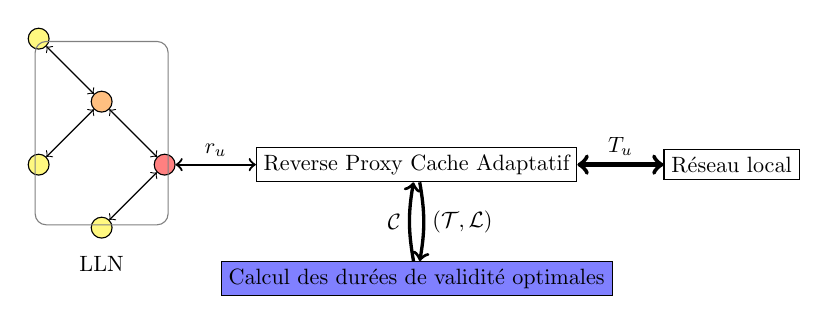
\begin{tikzpicture}[scale = .8, every node/.style={scale = .8}]

  % définition des styles
  \tikzstyle{visible}=[draw, fill=blue!50]
  \tikzstyle{hidden}=[ draw, fill=gray!20]
  \tikzstyle{router}=[circle, draw, fill=orange!50,text=black]
  \tikzstyle{child}=[circle, draw, fill=yellow!50,text=black]
  \tikzstyle{root}=[circle, draw, fill=red!50,text=black]

  % les nœuds
  \node[draw] (gw) {Reverse Proxy Cache Adaptatif};

  \node[visible, below=of gw] (adapt) {Calcul des durées de validité optimales};


  % Réseau contraint
  \node[root] (1) at (-4, 0) {};
  \node[router] (2) at (-5, 1) {};
  \node[child] (3) at (-5, -1) {};
  \node[child] (4) at (-6, 2) {};
  \node[child] (5) at (-6, 0) {};

  % \node[cloud, cloud puffs = 10, minimum width = 4cm, draw, fill = gray!10] (cloud) at (5,0) {Réseau local};
  \node[draw] (cloud) at (5,0) {Réseau local};

 \node [fit=(1) (2) (3) (4) (5), rounded corners, draw=black!50] (lln) {};
 \node [below=.3 cm of lln] {LLN};

\path

  % Réseau contraint
  (gw) edge[<->, thick] node [above] {$r_u$} (1)
  (1) edge[<->] (2)
  (1) edge[<->] (3)
  (2) edge[<->] (4)
  (2) edge[<->] (5)

  % Réseau conventionnel
  (gw.east) edge[<->, ultra thick] node [above] {$T_u$} (cloud)

  % Cache
  (gw) edge[->,very thick, bend left=10] node [midway,right] {$(\mathcal{T}, \mathcal{L})$} (adapt)
  (adapt) edge[->,very thick, bend left=10] node [left] {$\mathcal{C}$} (gw)
  ;

  \end{tikzpicture}
  \end{document}